\chapter{Seconda esercitazione}
\begin{figure}[htb]
    \centering
    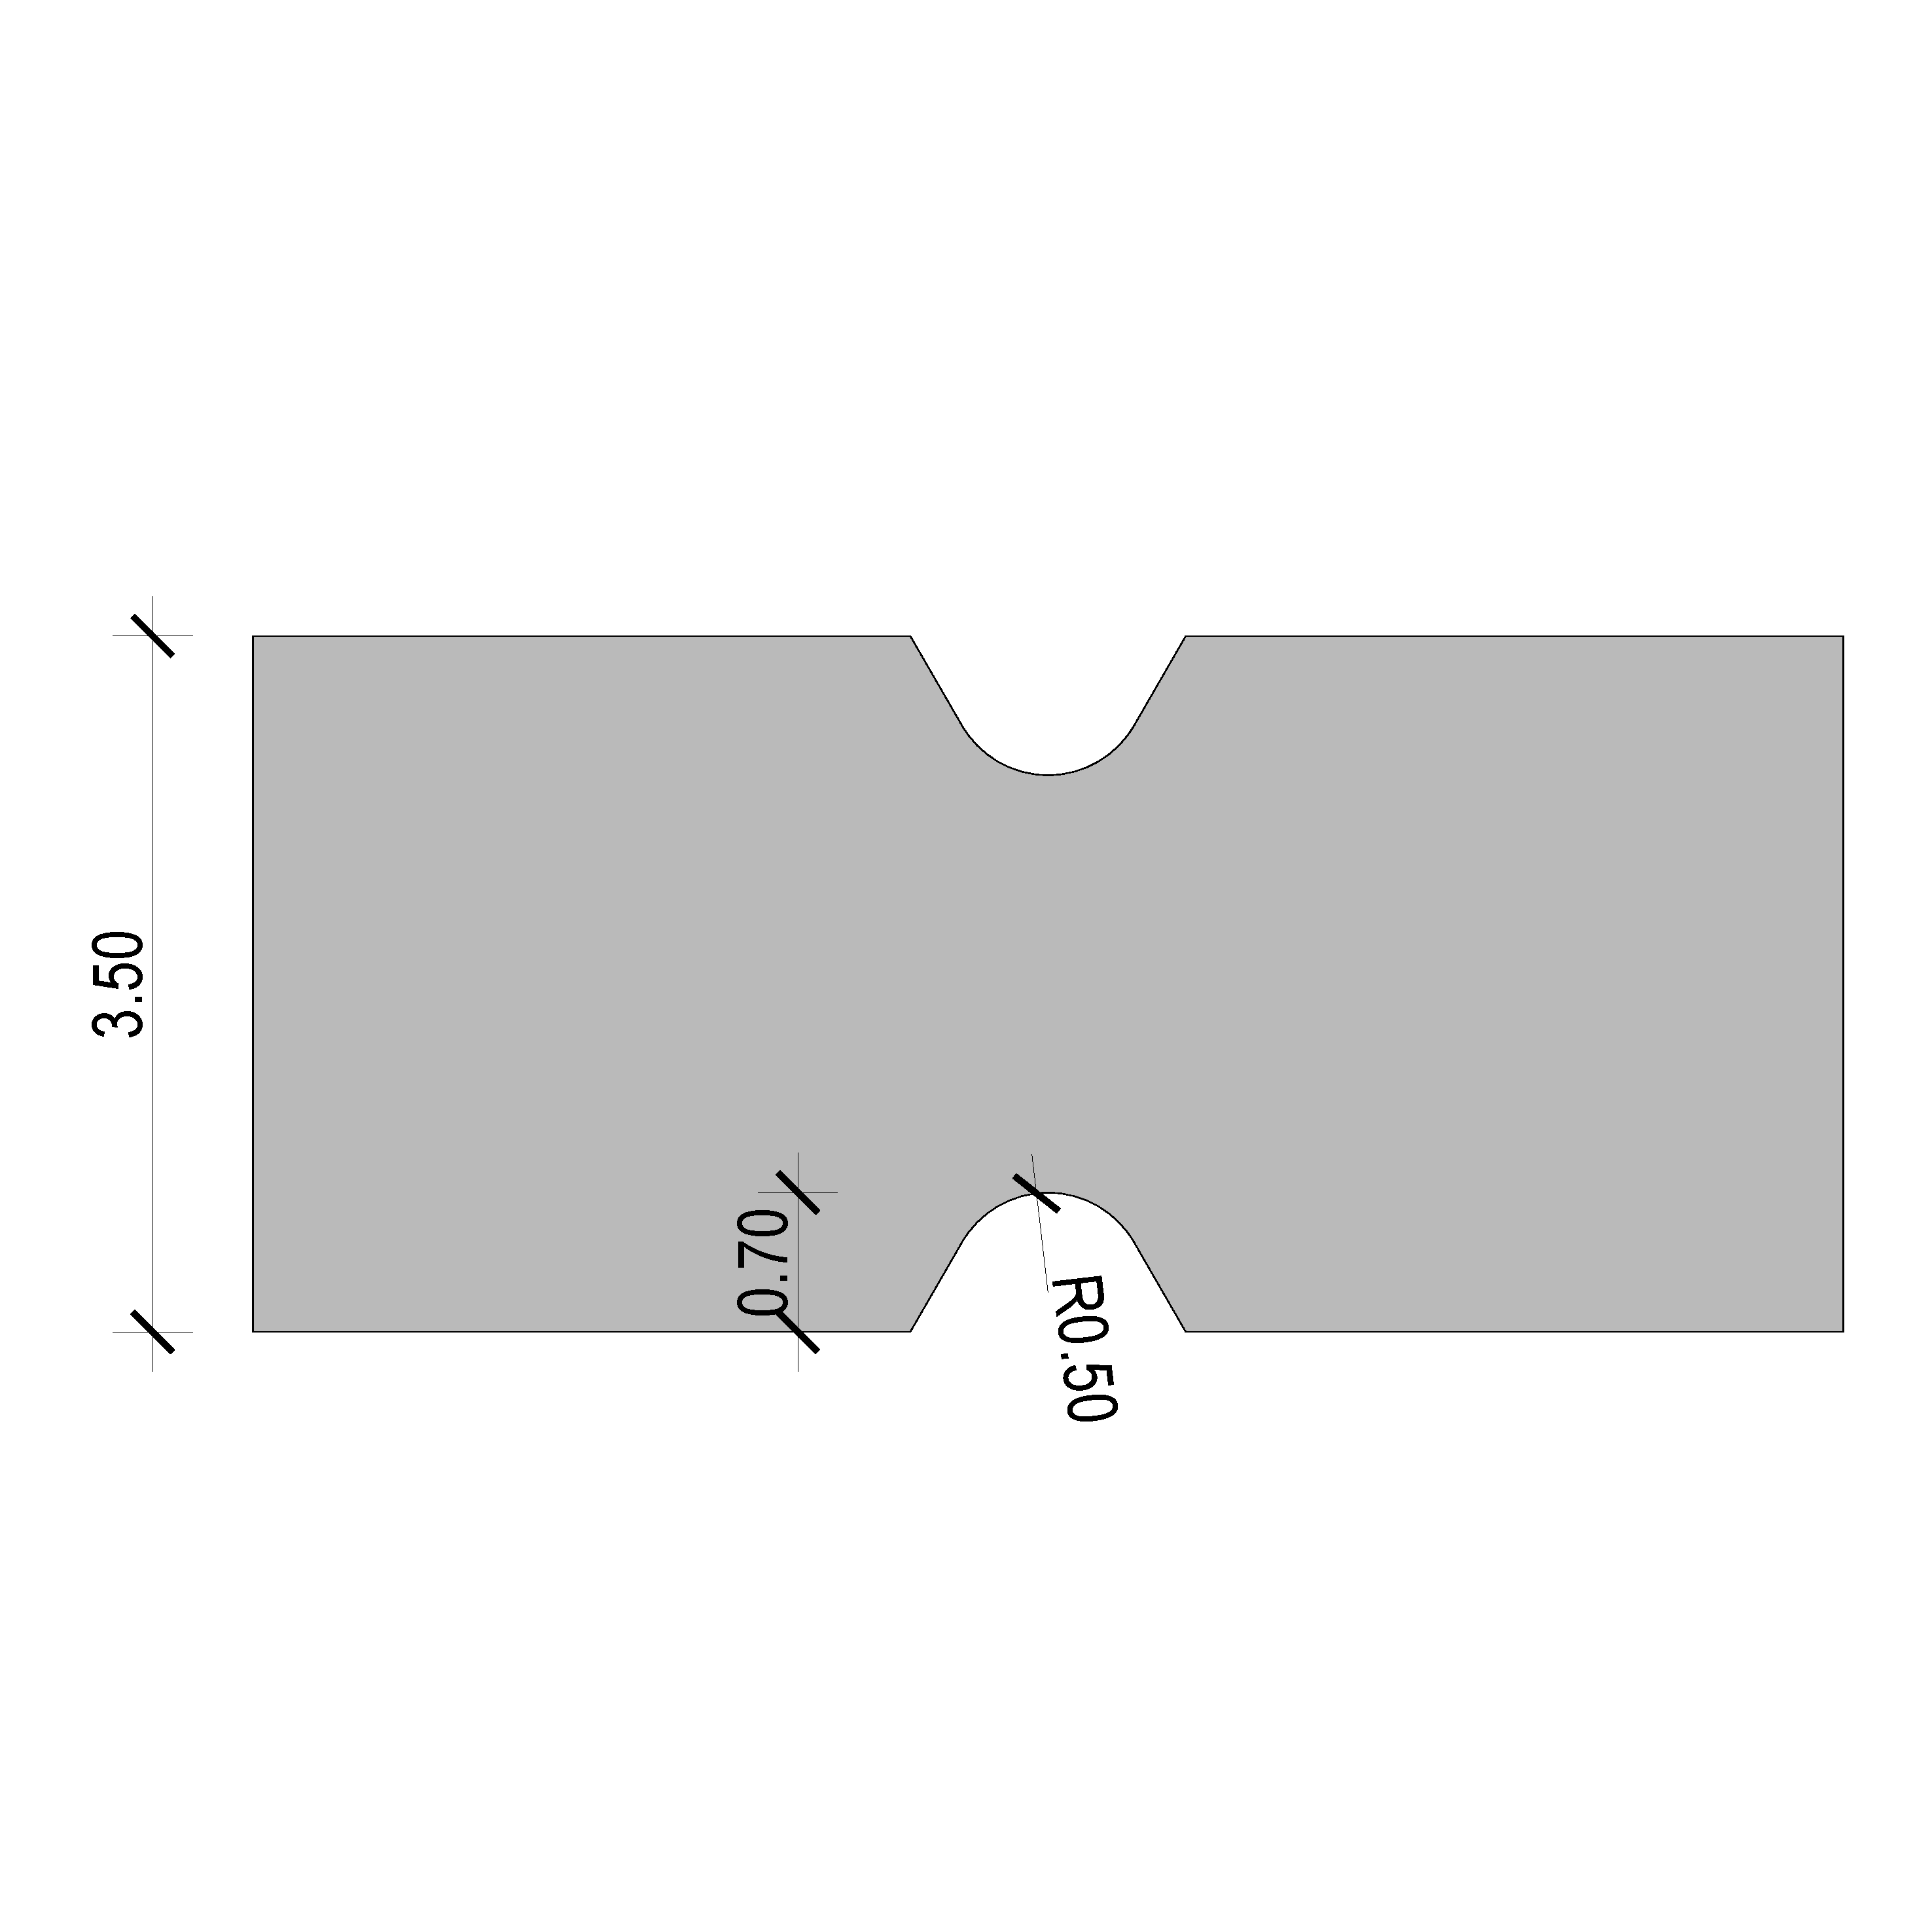
\includegraphics[width=0.9\textwidth]{rel2/img2/2Lastra.pdf}
    \caption{Lastra piana asseganata dall'esercitazione}
    \label{fig:lastraIniziale}
\end{figure}
La seconda esercitazione prevede lo studio con elementi finiti dello sforzo massimo alla quale viene sottoposta una lastra piana soggetta a trazione avente un particolare geometria raffigurata in figura \ref{fig:lastraIniziale}.

La soluzione è stata già calcolata analiticamente e viene riportato in letteratura il fattore di concentrazione degli sforzi $K_t$.
Nel caso di sforzi elastici con tensioni assiali e con fori a $V$ viene riportata la seguente soluzione
\begin{equation}\footnotesize\label{kt1}
K_0=\min
\begin{cases}
K_{t\theta}=K_{tu} & \\
K_{t\theta} = 1.11 K_{t\theta} - \left[0.0275 + 0.0001450 + 0.0164\left(\frac{\theta}{120}\right)^8\right]K_{t\theta}^2 & \text{se $\frac{2h}{D} = 0.40$ e $\theta\le \ang{120}$}\\
K_{t\theta} = 1.11 K_{t\theta} - \left[0.0275 + 0.000420 + 0.0075\left(\frac{\theta}{120}\right)^8\right]K_{t\theta}^2 & \text{se $\frac{2h}{D} = 0.667$ e $\theta\le \ang{120}$}
\end{cases}
\end{equation} 
mentre nel caso di fori a $U$ si ha
\begin{equation}\footnotesize\label{kt2}
K_t = C_1 + C_2\left(\frac{2h}{D}\right) + C_3\left(\frac{2h}{D}\right)^2 + C_4\left(\frac{2h}{D}\right)^3
\end{equation} 
dove 
\[ \footnotesize
\begin{array}{ccc}
\toprule
 & 0.1\le h/r\le 2.0 & 2.0\le h/r\le 50.0 \\ \midrule
C_1 & 0.850+2.628\sqrt{h/r}-0.413\,h/r & 0.833+2.069\sqrt{h/r}-0.009\,h/r \\ 
C_2 & -1.119-4.826\sqrt{h/r}+2.575\,h/r & 2.732-4.157\sqrt{h/r}+0.176\,h/r \\  
C_3 & 3.563-0.514\sqrt{h/r}-2.402\,h/r & -8.859+5.327\sqrt{h/r}-0.320\,h/r \\  
C_4 & -2.294 + 2.713\sqrt{h/r}+0.240\,h/r & 6.294-3.239\sqrt{h/r}+0.154\,h/r \\  \bottomrule
\end{array}
\]
Pertanto, combinando le due soluzioni \eqref{kt1} e \eqref{kt2} e utilizzando i dati della lastra, si ottiene:
\[
\begin{cases}
K_{tu}=2.10647\\
K_{t\theta}=2.17727
\end{cases} \implies K_t = K_{tu}
\]
Scegliendo uno sforzo $\sigma_1$ di \SI{50}{\mega\pascal} otteniamo uno sforzo $\sigma_{max}$ pari a \SI{175.539}{\mega\pascal}.
